\documentclass{ctexart}
\usepackage[T1]{fontenc}
\usepackage[a4paper,top=1.5cm,bottom=1.5cm,left=2cm,right=2cm,marginparwidth=1.75cm]{geometry}
\usepackage{mathtools}
\usepackage{tikz}
\usepackage{booktabs}
\usepackage{caption}
\usepackage{outlines}
\usepackage{graphicx}
\usepackage{amsthm}
\usepackage{minted}
\usepackage[colorlinks=false, allcolors=blue]{hyperref}
\renewcommand{\tableautorefname}{表}
\DeclarePairedDelimiter{\set}{\{}{\}}
\DeclarePairedDelimiter{\paren}{(}{)}
\graphicspath{ {./images/} }

\title{微机接口第五章作业}
\author{卢雨轩 19071125}
% \date{\today}
\ctexset{
    section = {
        titleformat = \raggedright,
        name = {,},
        number = \chinese{section}、
    },
    paragraph = {
        runin = false
    },
    today = small,
    figurename = 图,
    contentsname = 目录,
    tablename = 表,
}

\begin{document}

\maketitle

\begin{outline}[enumerate]
    \1 中断向量指什么,放在哪里?,对应8086的1CH的中断向量存放在哪里,如果1CH的中断处理程序从5110H:2030H开始,则中断向量应怎样存放?
    

    指中断处理程序的入口地址,放在IDT中。1CH * 4 = 70H,所以70H到73H的内容分别为30H,20H,10H,51H。

    \1 给定SP=0100H、SS=0500H、PSW=0240H,在存储单元中已有内容为(00024)=0060H、(00026)=1000H,在段地址为0800H及偏移地址为
    00A0H的单元中,有一条中断指令INT9。试问,执行INT9指令后,SS、SP、CS、IP、PSW的内容是什么?栈顶的三个字是什么?

    SS=0500H, SP= 00FAH, CS=1000H, IP = 0060H, PSW=0040H。
    栈顶的3个字为 00A2H, 0800H, 0240H。

    \1 假如外设A1、A2、A3、A4、A5按优先级排列,外设A1优先级最高,按下列提问,说明中断处理的运行次序,(中断服务程序中有STI指令)

    \2 外设A3,A4同时发中断请求;

    \2 外设A3中断处理中,外设A1发中断请求;

    \2 外设A1中断处理未完成前,发出EOI结束命令,外设A5发中断请求。

    \begin{center}
        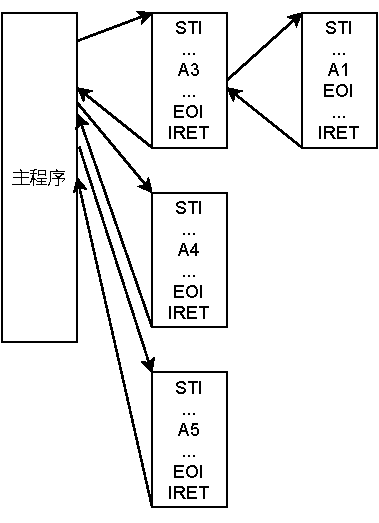
\includegraphics[width=0.4\textwidth]{3-image.pdf}
    \end{center}
\1 线路图中的电路有8086CPU、8255A、8259A、继电器及驱动和脉冲按钮UP组成。要求编写程序对IR0每次中断,去控制继电器动作,使LED闪烁。
\begin{minted}{gas}
START :MOV AL,13H;00010011B
        MOV DX,210H
        OUT DX,AL
        MOV AL,8
        MOV DX,211H
        OUT DX,AL
        MOV AL,01H
        OUT DX,AL
        MOV AX,0
        MOV DS,AX  
        LEA  AX,INT0
        MOV  DS:[4*8],AX
        MOV  AX,CS
        MOV  DS:[4*8+2],AX
        IN  AL,DX
        AND AL,0FEH        
        OUT DX,AL
        MOV DX,203H
        MOV AL,80H
        OUT DX,AL
        MOV BL,01H
        STI
LOP:    HLT 
        JMP  LOP

INT0    PROC NEAR 
        MOV DX,201H
        NOT BL
        MOV AL,BL
        OUT DX,AL
        MOV DX,210H
        MOV AL,20H
        OUT DX,AL
        IRET
        INT1 ENDP
\end{minted}
\1 某系统中有3片8259A级联使用,1片为8259A主片,2片为8259A从片,从片接入8259A主片的IR2和IR5端,并且当前8259A主片的IR3及两片8259A从片的IR4各接有一个外部中断源。中断类型基号分别为80H、90H、A0H、中断入口段基址在2000H,偏移地址分别为1800H、2800H、3800H、主片8259A的端口地址为CCF8H、CCFAH。一片8259A从片的端口地址为FEE8H、FEEAH,另一片为FEECH、FEEEH。中断采用电平触发,完全嵌套工作方式,普通EOI结束。

\2 画出硬件连接图;

\2 编写初始化程序。
\begin{minted}{gas}
    MOV DX, CCF8H
    MOV AL, 19H
    OUT DX, AL
    MOV DX, CCFAH
    MOV AL, 80H
    OUT DX, AL
    MOV AL, 24H
    OUT DX, AL
    MOV AL, 11H
    OUT DX, AL
    MOV AL, D3H
    OUT DX, AL
    MOV DX, CCF8H
    MOV AL, 20H
    OUT DX, AL

    MOV DX, FEE8H
    MOV AL, 19H
    OUT DX, AL
    MOV DX, FEEAH
    MOV AL, 90H
    OUT DX, AL
    MOV AL, 02H
    OUT DX, AL
    MOV AL, 01H
    OUT DX, AL
    MOV AL, EFH
    OUT DX, AL
    MOV DX, FEE8H
    MOC AL, 20H
    OUT DX, AL

    MOV DX, FEECH
    MOV AL, 19H
    OUT DX, AL
    MOV DX, FEEEH
    MOV AL, 90H
    OUT DX, AL
    MOV AL, 05H
    OUT DX, AL
    MOV AL, 01H
    OUT DX, AL
    MOV AL, EFH
    OUT DX, AL
    MOV DX, FEECH
    MOC AL, 20H
    OUT DX, AL



\end{minted}

\end{outline}

\end{document}
